\part{Omega Axioms and Hilbert Space Geometry}
\label{part:II}

\section{The Omega Axiom and Geometric Time}
\label{chap:omega_axiom}

\subsection{Axiom O1: The Static Universe Vector}
We begin with the most radical yet simplest postulate of the theory.

\begin{axiom}[The Omega Axiom]
The physical universe is ontologically isomorphic to a single, unique, normalized vector $|\Omega\rangle$ in an infinite-dimensional, separable complex Hilbert space $\mathcal{H}$. This state is timeless in the absolute sense:
\begin{equation}
    \frac{\partial}{\partial t_{\text{ext}}} |\Omega\rangle \equiv 0.
\end{equation}
There is no external time parameter $t_{\text{ext}}$. The "state of the universe" does not change; it simply \textit{is}.
\end{axiom}

\subsection{Intrinsic Time from Spectral Decomposition}
If the universe is static, whence comes the illusion of change? Time is emergent. It is defined internally by comparing the static vector $|\Omega\rangle$ against a reference basis.
Let $\hat{H}$ be a self-adjoint operator (the Hamiltonian) defining an orthogonal basis $\{|E_n\rangle\}$. The vector $|\Omega\rangle$ can be decomposed as:
\begin{equation}
    |\Omega\rangle = \sum_n c_n |E_n\rangle, \quad \sum_n |c_n|^2 = 1.
\end{equation}
We define a 1-parameter family of states $|\Omega(\tau)\rangle$ by injecting a phase factor relations to the basis energies:
\begin{equation}
    |\Omega(\tau)\rangle \equiv \sum_n c_n e^{-\iu E_n \tau} |E_n\rangle.
\end{equation}

\subsubsection{Intrinsic phase-orbit coding and Zeckendorf time}
The intrinsic parameter $\tau$ serves as a coordinate parametrizing a curve $\mathcal{C}$ in the unit sphere of $\mathcal{H}$ (and hence a trajectory in the projective space $\mathbb{P}(\mathcal{H})$). To connect this continuous intrinsic evolution to a discrete computational clock, we introduce a canonical one-dimensional phase readout of the intrinsic phase orbit.

\begin{definition}[Intrinsic phase-orbit readout]
Fix a reference vector $|r\rangle\in\mathcal{H}$ such that $\langle r|\Omega(\tau)\rangle\neq 0$ for the times of interest (e.g., $|r\rangle=|E_0\rangle$ with $c_0\neq 0$). Define the phase readout
\begin{equation}
    x(\tau)\ \equiv\ \frac{1}{2\pi}\arg\langle r|\Omega(\tau)\rangle\ \ \bmod 1,
\end{equation}
which maps the intrinsic phase orbit to a circle variable $x(\tau)\in\mathbb{R}/\mathbb{Z}$.
\end{definition}

\begin{definition}[Circle-rotation sampling and Sturmian coding]
Let $t\in\mathbb{Z}_{\ge 0}$ index discrete ticks (e.g., QCA steps) and sample $x(\tau)$ stroboscopically as $x_t\equiv x(\tau_0+t\Delta\tau)$. In the irrational-rotation regime this is modeled as
\begin{equation}
    x_{t+1}=x_t+\alpha \pmod 1,\qquad \alpha\in(0,1)\setminus\mathbb{Q}.
\end{equation}
Partition the circle into two intervals
\begin{equation}
    I_L=[0,1-\alpha),\qquad I_S=[1-\alpha,1),
\end{equation}
and define the symbolic coding $\sigma_t\in\{L,S\}$ by
\begin{equation}
    \sigma_t=
    \begin{cases}
    L,& x_t\in I_L,\\
    S,& x_t\in I_S.
    \end{cases}
\end{equation}
Such codings of irrational rotations are Sturmian sequences; for the golden-slope choice $\alpha=\phi^{-2}$ (with $\phi=\tfrac{1+\sqrt5}{2}$), $\{\sigma_t\}$ is the Fibonacci word \cite{MorseHedlund1940,Lothaire2002}.
\end{definition}

\begin{proposition}[Ostrowski numeration and the Zeckendorf specialization (golden case)]
For an irrational slope $\alpha$, the associated Ostrowski numeration gives a unique digit expansion of each integer time $t$. In the golden case $\alpha=\phi^{-2}$, this admissibility condition reduces to the Zeckendorf rule (no consecutive Fibonacci summands): writing the Fibonacci numbers as $F_0=0$, $F_1=1$, $F_{n+2}=F_{n+1}+F_n$, every $t\in\mathbb{Z}_{\ge 0}$ admits a unique expansion
\begin{equation}
    t=\sum_{k\ge 0} b_k F_{k+2},\qquad b_k\in\{0,1\},\qquad b_k b_{k+1}=0,
\end{equation}
and conversely every such digit string represents a unique integer \cite{Zeckendorf1972,AlloucheShallit2003}.
\end{proposition}

\noindent\textit{Interpretation.} The intrinsic phase orbit can be read out as a canonical Fibonacci (Long/Short) symbol stream and, equivalently, a Zeckendorf-addressable digit structure for discrete ticks. This provides a natural intrinsic clock and a sparse hierarchical schedule for activating scale-dependent updates.

\subsection{The Fubini-Study Metric as Physical Duration}
To give $\tau$ a geometric meaning independent of the specific parametrization, we employ the natural metric of the projective Hilbert space $\mathbb{P}(\mathcal{H})$: the Fubini-Study metric.
For two infinitesimally close states $|\psi\rangle$ and $|\psi + d\psi\rangle$, the distance $ds$ is:
\begin{equation}
    ds^2 = \langle d\psi | d\psi \rangle - |\langle \psi | d\psi \rangle|^2 = \left( \langle \hat{H}^2 \rangle - \langle \hat{H} \rangle^2 \right) d\tau^2 = (\Delta H)^2 d\tau^2.
\end{equation}
This yields the fundamental relation between geometry and dynamics.
\begin{theorem}[Anandan-Aharonov Relation]
The speed of evolution of a quantum state in the projective Hilbert space $\mathbb{P}(\mathcal{H})$ is strictly determined by the energy uncertainty (standard deviation of the Hamiltonian) \cite{Anandan1990}:
\begin{equation}
    v_{\tau} = \frac{ds}{d\tau} = \frac{2}{\hbar} \Delta H = \frac{2}{\hbar} \sqrt{\langle \hat{H}^2 \rangle - \langle \hat{H} \rangle^2}.
\end{equation}
\end{theorem}
This interprets "Time" not as a coordinate but as a statistical distance. Time flows only because the universe is \textit{not} an eigenstate of its own Hamiltonian ($\Delta E > 0$). If $\Delta E = 0$ (Heat Death), time stops ($v_{\tau} = 0$).

\subsection{Comparison with Page-Wootters Formalism}
Our approach resonates with the Page-Wootters mechanism \cite{PageWootters1983}, where time is a correlation between a clock subsystem and the rest of the universe. However, we do not arbitrarily partition $\mathcal{H}$ into $\mathcal{H}_{\text{clock}} \otimes \mathcal{H}_{\text{sys}}$. Instead, time is a global property of the spectral distribution of the entire state $|\Omega\rangle$.

\section{Finite Information, Locality, and Holography}
\label{chap:axioms_structure}

\subsection{Axiom O2: Finite Information}
Formal quantum mechanics allows for infinite information density (e.g., distinguishing $|x\rangle$ from $|x+\epsilon\rangle$). However, the Bekenstein bound implies nature does not support this.

\begin{axiom}[Finite Information Axiom]
For any causally closed region with boundary area $A$, the dimension of its effective Hilbert space is finite:
\begin{equation}
    \dim \mathcal{H}_{\text{region}} = \exp\left(\frac{A}{4 l_P^2}\right).
\end{equation}
Consequently, we take the microscopic description to admit a decomposition into finite-dimensional local factors. Continuous variables (fields, coordinates) are emergent approximations.
\end{axiom}

\subsection{Remark: Local operator algebras and approximate factorization}
In continuum relativistic QFT, the operator algebra associated with a bounded region is typically a type~III von Neumann algebra, and an exact tensor factorization $\mathcal{H}\simeq \mathcal{H}_R \otimes \mathcal{H}_{R^c}$ is not available; this is closely tied to the ultraviolet structure and divergent entanglement at sharp boundaries (see, e.g., \cite{Haag1996}). Omega Theory takes Axiom~O2 as indicating a fundamentally regulated description with finite information per causal region, for which local algebras are type~I and tensor factorization is meaningful at the microscopic level.

The continuum QFT description is interpreted as an effective scaling limit in which type~III behavior is recovered. In that limit, an approximate tensor-product structure can be formulated using the \textbf{split property}: for nested regions $R \subset R_{\epsilon}$ there exists an intermediate type~I factor that enables a controlled notion of localization and effective subsystem Hilbert spaces \cite{Buchholz1987}. Throughout this manuscript, statements such as $\mathcal{H}=\bigotimes_{v\in V}\mathcal{H}_v$ should therefore be read as microscopic/regulated constructions, not as a claim about exact factorization in continuum QFT.

\begin{figure}[ht]
    \centering
    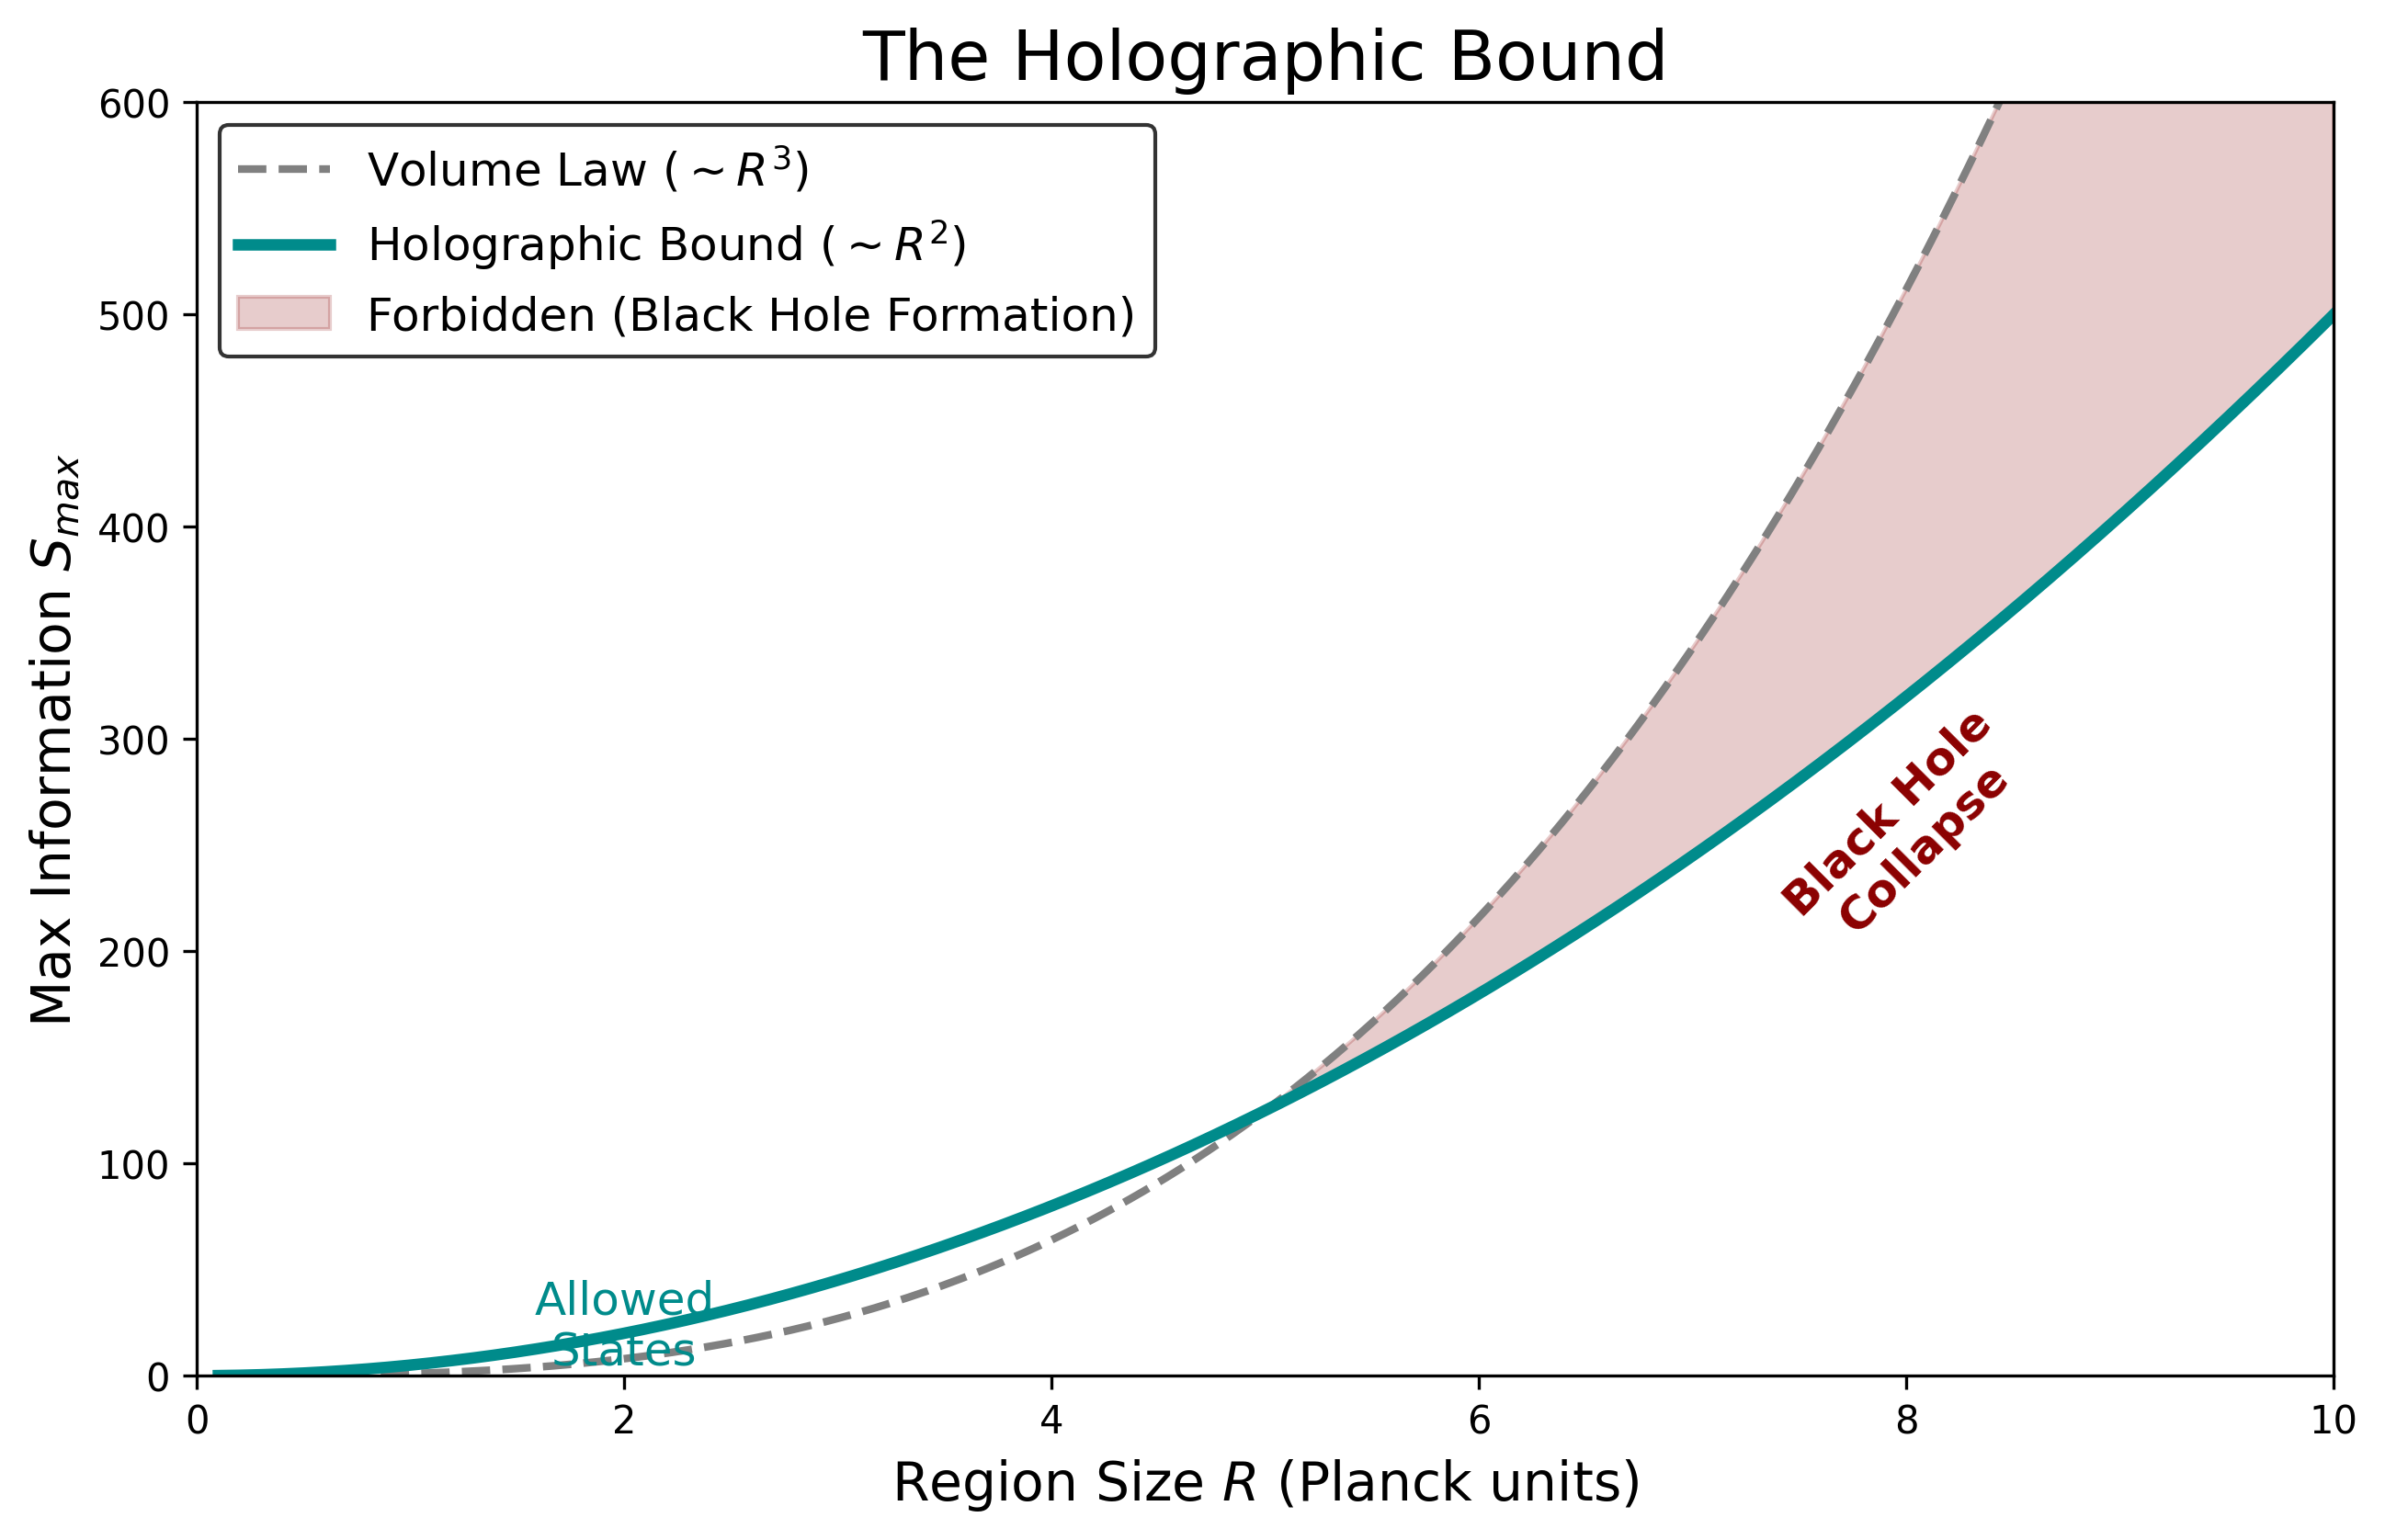
\includegraphics[width=0.8\linewidth]{images/holographic_scaling.png}
    \caption{\textbf{The Holographic Bound}. Comparison between extensive Volume Law scaling ($S \sim R^3$, dashed gray) which leads to black hole formation, and the Holographic Area Law ($S \sim R^2$, solid cyan) which represents the physical limit of information density.}
    \label{fig:holography}
\end{figure}

\subsection{Axiom O3: Causal Locality}
To define "region" and "area" without a pre-existing manifold, we need a graph structure.
\begin{axiom}[Causal Locality Axiom]
The microscopic Hilbert space decomposes as $\mathcal{H} = \bigotimes_{v \in V} \mathcal{H}_v$ over a countable graph $G=(V, E)$. The evolution operator $\hat{U}$ factorizes into local gates acting only on connected vertices.
\begin{equation}
    \hat{U} = \prod_{k} \hat{U}_k^{\text{local}}.
\end{equation}
This locality imposes a strict "light cone" structure on the propagation of information, recovering the causal structure of Special Relativity in the continuum limit.
\end{axiom}

\subsection{Axiom O4: The Holographic Mapping}
\begin{axiom}[Holographic Mapping Axiom]
Let $\mathcal{H}_{\text{bulk}}$ be the Hilbert space of the bulk QCA on the graph $G$, and $\mathcal{H}_{\partial G}$ be the Hilbert space associated with the graph boundary $\partial G$. We postulate the existence of a holographic isometry $\Phi: \mathcal{H}_{\text{bulk}} \hookrightarrow \mathcal{H}_{\partial G}$ that maps bulk states to boundary states.

\textbf{Concrete Construction (Golden MERA)}: The isometry $\Phi$ is strictly defined by the renormalization group flow of the Quasicrystal. Let $\{\Lambda_s\}_{s=0}^{N}$ be a hierarchy of tilings where $\Lambda_{s+1}$ is generated from $\Lambda_s$ via the standard inflation rule (e.g., $L \to L+S, S \to L$ for 1D, or the equivalent Penrose substitution). The mapping is constructed as a tensor network:
\begin{equation}
    \Phi \equiv \lim_{N \to \infty} \prod_{s=0}^{N} \left( \hat{D}_s \cdot \hat{W}_s \right),
\end{equation}
where $\hat{W}_s$ are isometric "inflation tensors" and $\hat{D}_s$ are local unitary "disentanglers". In Appendix \ref{app:isometry}, we formalize the construction under a perfect-tensor (or $\epsilon$-perfect) assumption and derive the corresponding recoverability conditions.

\paragraph{Zeckendorf addressing of inflation layers.}
In the 1D golden case, the inflation hierarchy admits a canonical arithmetic addressing by Zeckendorf digits: for an integer position (or coarse-graining address) $x\in\mathbb{Z}_{\ge 0}$ one may write uniquely
\begin{equation}
    x=\sum_{k\ge 0} b_k F_{k+2},\qquad b_k\in\{0,1\},\qquad b_k b_{k+1}=0.
\end{equation}
The digit $b_k$ indicates whether scale layer $k$ contributes a long-scale threshold in the inflation history of that site, providing a sparse hierarchical label for causal structure in the Golden MERA. In this sense, Fibonacci fusion fixes the local tensor data (Appendix \ref{app:formal_proofs}), while Zeckendorf addressing fixes a canonical scheduling/labeling of discrete scale events \cite{Zeckendorf1972,AlloucheShallit2003}.

\textbf{Error Correction and Recovery}: This tensor network functions as a Quantum Error Correcting Code (QECC).
\begin{enumerate}
    \item \textbf{Complementary Recovery}: For any boundary region $R$, the bulk operators in the \textit{entanglement wedge} $\mathcal{W}_E(R)$ can be reconstructed as operators on $R$. Theorem \ref{app:isometry} (Entanglement Wedge Reconstruction) proves that $\Phi \hat{O}_{\text{bulk}} \Phi^\dagger = \hat{O}_R \otimes \hat{I}_{\bar{R}} + \mathcal{E}$.
    \item \textbf{Code Distance}: The topological protection of the bulk is guaranteed by the code distance $d \sim L^{\frac{1}{\phi}}$. The error term $\mathcal{E}$ is exponentially suppressed as $e^{-d \cdot \ln \chi}$ (see Proposition \ref{prop:error_suppression} in Appendix \ref{app:isometry}).
\end{enumerate}

\subsection{The Factorization Problem and Baby Universes}
A central puzzle in modern holography is the "Factorization Problem" \cite{Harlow2021}: in a theory with multiple boundaries, the gravitational path integral (which includes connected topologies like Euclidean wormholes) fails to factorize, suggesting an ensemble average over dual theories rather than a single unitary description. This is formalized by the inclusion of "Baby Universes" or $\alpha$-parameters in the Hilbert space.

Omega Theory offers a definitive resolution: the "Alpha Parameters" correspond to the fixed, unique spectral data of the global state $|\Omega\rangle$. By positing a single, rigid vector rather than a statistical ensemble, we effectively "fix the gauge" of the baby universe Hilbert space. Spacetime wormholes are not fundamental topology changes but rather non-local entanglement correlations within the unique tensor network. Factorization is restored because the theory is fundamentally a single quantum system, not an average over random Hamiltonians (as in SYK).

The geometric area law follows from this structure: for a state $|\psi\rangle$ defined by this network, the entropy $S(\rho_R)$ is upper-bounded by the number of bond cuts required to sever $R$ from the rest of the network, which scales as the area of the minimal surface $\gamma_R$:
\begin{equation}
    S(\rho_R) \propto |\text{min-cut}(R)| \sim \frac{\text{Area}(\gamma_R)}{4 l_P^2}.
\end{equation}
\end{axiom}
